DTMF is a signaling system that is used to
transmit numbers and characters. The original purpose of the system
was to transmit numbers entered by a caller.
The aim the exercise was to analyse a given DTMF signal by
creating a function which recognises the numbers in the signal
automatically.

The DTMF system works by sending signals at two different
frequencies. Each transmitted number corresponds to an unique
letter. For example the frequencies 770 Hz and 1336 Hz together
represent the number 5.

It was given in the exercise that each number is at least
70ms long and there is a pause of at least 40ms between each number. We
ended up using a 20ms sized window since this guarantees, that
there is at least one silent window between the numbers.
We differentiate the numbers using this silent window.

The flow of the program is as follows: for each window, the energy of the
window is calculated. If the energy exceeds a hard coded
threshold of 0.0001, we assume that the window constains an
actual signal. If the threshold is exceeded, we calculate
the amplitude response of the signal, an example of which is depicted in
figure \ref{fig:q2_amplitude_response}.


\begin{figure}[h!]
  \begin{center}
    \hspace*{-1in}
    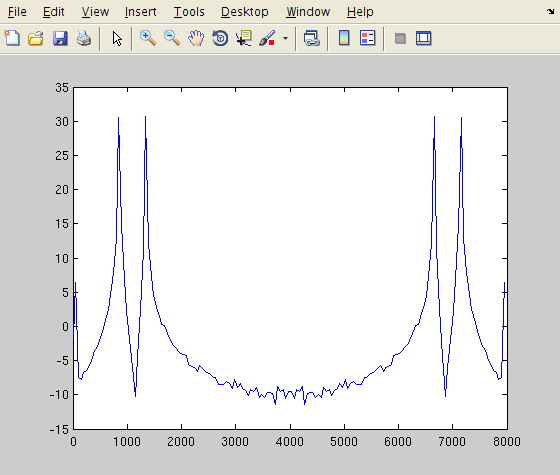
\includegraphics[width=100mm]{Q2/magnitude_vs_freq.png}
    \caption{The amplitude response of the signal. 
      \label{fig:q2_amplitude_response}}
  \end{center}  
\end{figure}


In the figure it is easy to see the two frequencies which
contain the information about the number being transmitted.
The program finds the two peaks scanning through the frequency spectrum
and taking the first value that exceeds the threshold, then scanning
ahead until the specturm goes under the threashold and then taking the
first value to exceed the threshold again. Then the program rounds
the two found frequencies to the nearest matching  DTMF frequency and
translates them into the corresponding number. Once the number has been
decoded, the program waits for the next silent window.

The program gave correct results for the given signal
\verb|dtmf_81231H-wav|,
but when it was tested with the 12 test signals,
it was only able to get 6 signals perfectly decoded.

It could be possible to improve the program by tuning the
hard coded thresholds better and using a more sophisticated
method for detecting the peaks. We could also
consider all 20ms windows
of the signal, not just the first one.

